\chapter{CHUYỂN ĐỔI SANG LƯỢC ĐỒ QUAN HỆ VÀ CHUẨN HÓA BCNF}

\section{Quy tắc ánh xạ từ lược đồ thực thể liên kết sang mô hình quan hệ}

Quá trình chuyển đổi từ lược đồ thực thể liên kết sang các lược đồ quan hệ được thực hiện theo các quy tắc sau:
\begin{enumerate}
    \item \textbf{Ánh xạ tập thực thể mạnh}: Mỗi tập thực thể mạnh gồm \texttt{SAN\_VAN\_DONG}, \texttt{DOI\_BONG}, \texttt{CAU\_THU}, \texttt{TRONG\_TAI}, \texttt{VONG\_DAU} được chuyển thành một quan hệ độc lập. Khóa chính của thực thể trở thành khóa chính của quan hệ tương ứng.
    \item \textbf{Ánh xạ mối kết hợp một -- nhiều}: Được chuyển đổi bằng cách lấy thuộc tính khóa chính của quan hệ phía bên một đưa vào làm thuộc tính khóa ngoại tại quan hệ phía bên nhiều. Ví dụ: Thuộc tính \texttt{MaSanNha} trong quan hệ \texttt{DOI\_BONG} là khóa ngoại tham chiếu đến khóa chính \texttt{MaSan} của quan hệ \texttt{SAN\_VAN\_DONG}.
    \item \textbf{Ánh xạ thuộc tính đa trị và thực thể yếu}: Thuộc tính màu áo của đội bóng được tách thành bảng riêng \texttt{MAU\_AO\_DOI\_BONG}. Khóa chính tổ hợp gồm thuộc tính khóa của đội bóng \texttt{MaDoi} và thuộc tính phân biệt \texttt{LoaiMauAo}.
    \item \textbf{Ánh xạ mối kết hợp nhiều -- nhiều}: Mối kết hợp nhiều -- nhiều giữa \texttt{TRAN\_DAU} và \texttt{TRONG\_TAI} được tách thành quan hệ trung gian \texttt{PHAN\_CONG\_TRONG\_TAI} với khóa chính tổ hợp gồm \texttt{MaTran} và \texttt{VaiTro}. Tương tự, danh sách thi đấu được biểu diễn qua quan hệ \texttt{DANG\_KY\_THI\_DAU}.
\end{enumerate}

\section{Tập hợp các lược đồ quan hệ và liên kết khóa}

Sau khi ánh xạ, hệ thống gồm 11 lược đồ quan hệ. Ký hiệu quy ước: Thuộc tính \underline{\textbf{in đậm gạch chân}} là khóa chính, thuộc tính \textit{in nghiêng} là khóa ngoại.

\begin{enumerate}
    \item $\text{SAN\_VAN\_DONG}(\underline{\mathbf{MaSan}}, \text{TenSan}, \text{DiaChi}, \text{SucChua})$
    
    \item $\text{DOI\_BONG}(\underline{\mathbf{MaDoi}}, \text{TenDoi}, \text{HLV}, \textit{MaSanNha})$\\
    \textit{Khóa ngoại: $\text{MaSanNha} \rightarrow \text{SAN\_VAN\_DONG}(\text{MaSan})$}
    
    \item $\text{MAU\_AO\_DOI\_BONG}(\underline{\mathbf{MaDoi}}, \underline{\mathbf{LoaiMauAo}}, \text{MoTaMau})$\\
    \textit{Khóa ngoại: $\text{MaDoi} \rightarrow \text{DOI\_BONG}(\text{MaDoi})$}
    
    \item $\text{CAU\_THU}(\underline{\mathbf{MaCauThu}}, \text{HoTen}, \text{NgaySinh}, \text{ViTri}, \text{QuocTich})$
    
    \item $\text{HOP\_DONG\_CAU\_THU}(\underline{\mathbf{MaHD}}, \textit{MaCauThu}, \textit{MaDoiChuQuan}, \textit{MaDoiHienTai}, \text{SoAo}, \text{NgayBatDau}, \text{NgayKetThuc}, \text{TrangThai}, \text{MucLuong})$\\
    \textit{Khóa ngoại: $\text{MaCauThu} \rightarrow \text{CAU\_THU}(\text{MaCauThu})$}\\
    \textit{Khóa ngoại: $\text{MaDoiChuQuan} \rightarrow \text{DOI\_BONG}(\text{MaDoi})$}\\
    \textit{Khóa ngoại: $\text{MaDoiHienTai} \rightarrow \text{DOI\_BONG}(\text{MaDoi})$}
    
    \item $\text{TRONG\_TAI}(\underline{\mathbf{MaTrongTai}}, \text{HoTen}, \text{NgaySinh}, \text{QueQuan}, \text{CapBac})$
    
    \item $\text{VONG\_DAU}(\underline{\mathbf{MaVong}}, \text{TenVong}, \text{ThuTu})$
    
    \item $\text{TRAN\_DAU}(\underline{\mathbf{MaTran}}, \textit{MaVong}, \textit{MaDoiNha}, \textit{MaDoiKhach}, \textit{MaSan}, \text{NgayGio}, \text{GiaVe}, \text{SoKhach}, \text{BanThangNha}, \text{BanThangKhach}, \text{TheVangNha}, \text{TheVangKhach}, \text{TheDoNha}, \text{TheDoKhach}, \text{TrangThai})$\\
    \textit{Khóa ngoại: $\text{MaVong} \rightarrow \text{VONG\_DAU}(\text{MaVong})$}\\
    \textit{Khóa ngoại: $\text{MaDoiNha} \rightarrow \text{DOI\_BONG}(\text{MaDoi})$}\\
    \textit{Khóa ngoại: $\text{MaDoiKhach} \rightarrow \text{DOI\_BONG}(\text{MaDoi})$}\\
    \textit{Khóa ngoại: $\text{MaSan} \rightarrow \text{SAN\_VAN\_DONG}(\text{MaSan})$}
    
    \item $\text{PHAN\_CONG\_TRONG\_TAI}(\underline{\mathbf{MaTran}}, \underline{\mathbf{VaiTro}}, \textit{MaTrongTai})$\\
    \textit{Khóa ngoại: $\text{MaTran} \rightarrow \text{TRAN\_DAU}(\text{MaTran})$}\\
    \textit{Khóa ngoại: $\text{MaTrongTai} \rightarrow \text{TRONG\_TAI}(\text{MaTrongTai})$}
    
    \item $\text{DANG\_KY\_THI\_DAU}(\underline{\mathbf{MaTran}}, \underline{\mathbf{MaCauThu}}, \textit{MaDoi}, \text{LoaiDangKy}, \text{SoAoTran})$\\
    \textit{Khóa ngoại: $\text{MaTran} \rightarrow \text{TRAN\_DAU}(\text{MaTran})$}\\
    \textit{Khóa ngoại: $\text{MaCauThu} \rightarrow \text{CAU\_THU}(\text{MaCauThu})$}\\
    \textit{Khóa ngoại: $\text{MaDoi} \rightarrow \text{DOI\_BONG}(\text{MaDoi})$}
    
    \item $\text{SU\_KIEN\_TRAN\_DAU}(\underline{\mathbf{MaSuKien}}, \textit{MaTran}, \textit{MaCauThu}, \textit{MaDoi}, \text{LoaiSuKien}, \text{PhutGhiNhan})$\\
    \textit{Khóa ngoại: $\text{MaTran} \rightarrow \text{TRAN\_DAU}(\text{MaTran})$}\\
    \textit{Khóa ngoại: $\text{MaCauThu} \rightarrow \text{CAU\_THU}(\text{MaCauThu})$}\\
    \textit{Khóa ngoại: $\text{MaDoi} \rightarrow \text{DOI\_BONG}(\text{MaDoi})$}
\end{enumerate}

\begin{figure}[H]
	\centering
	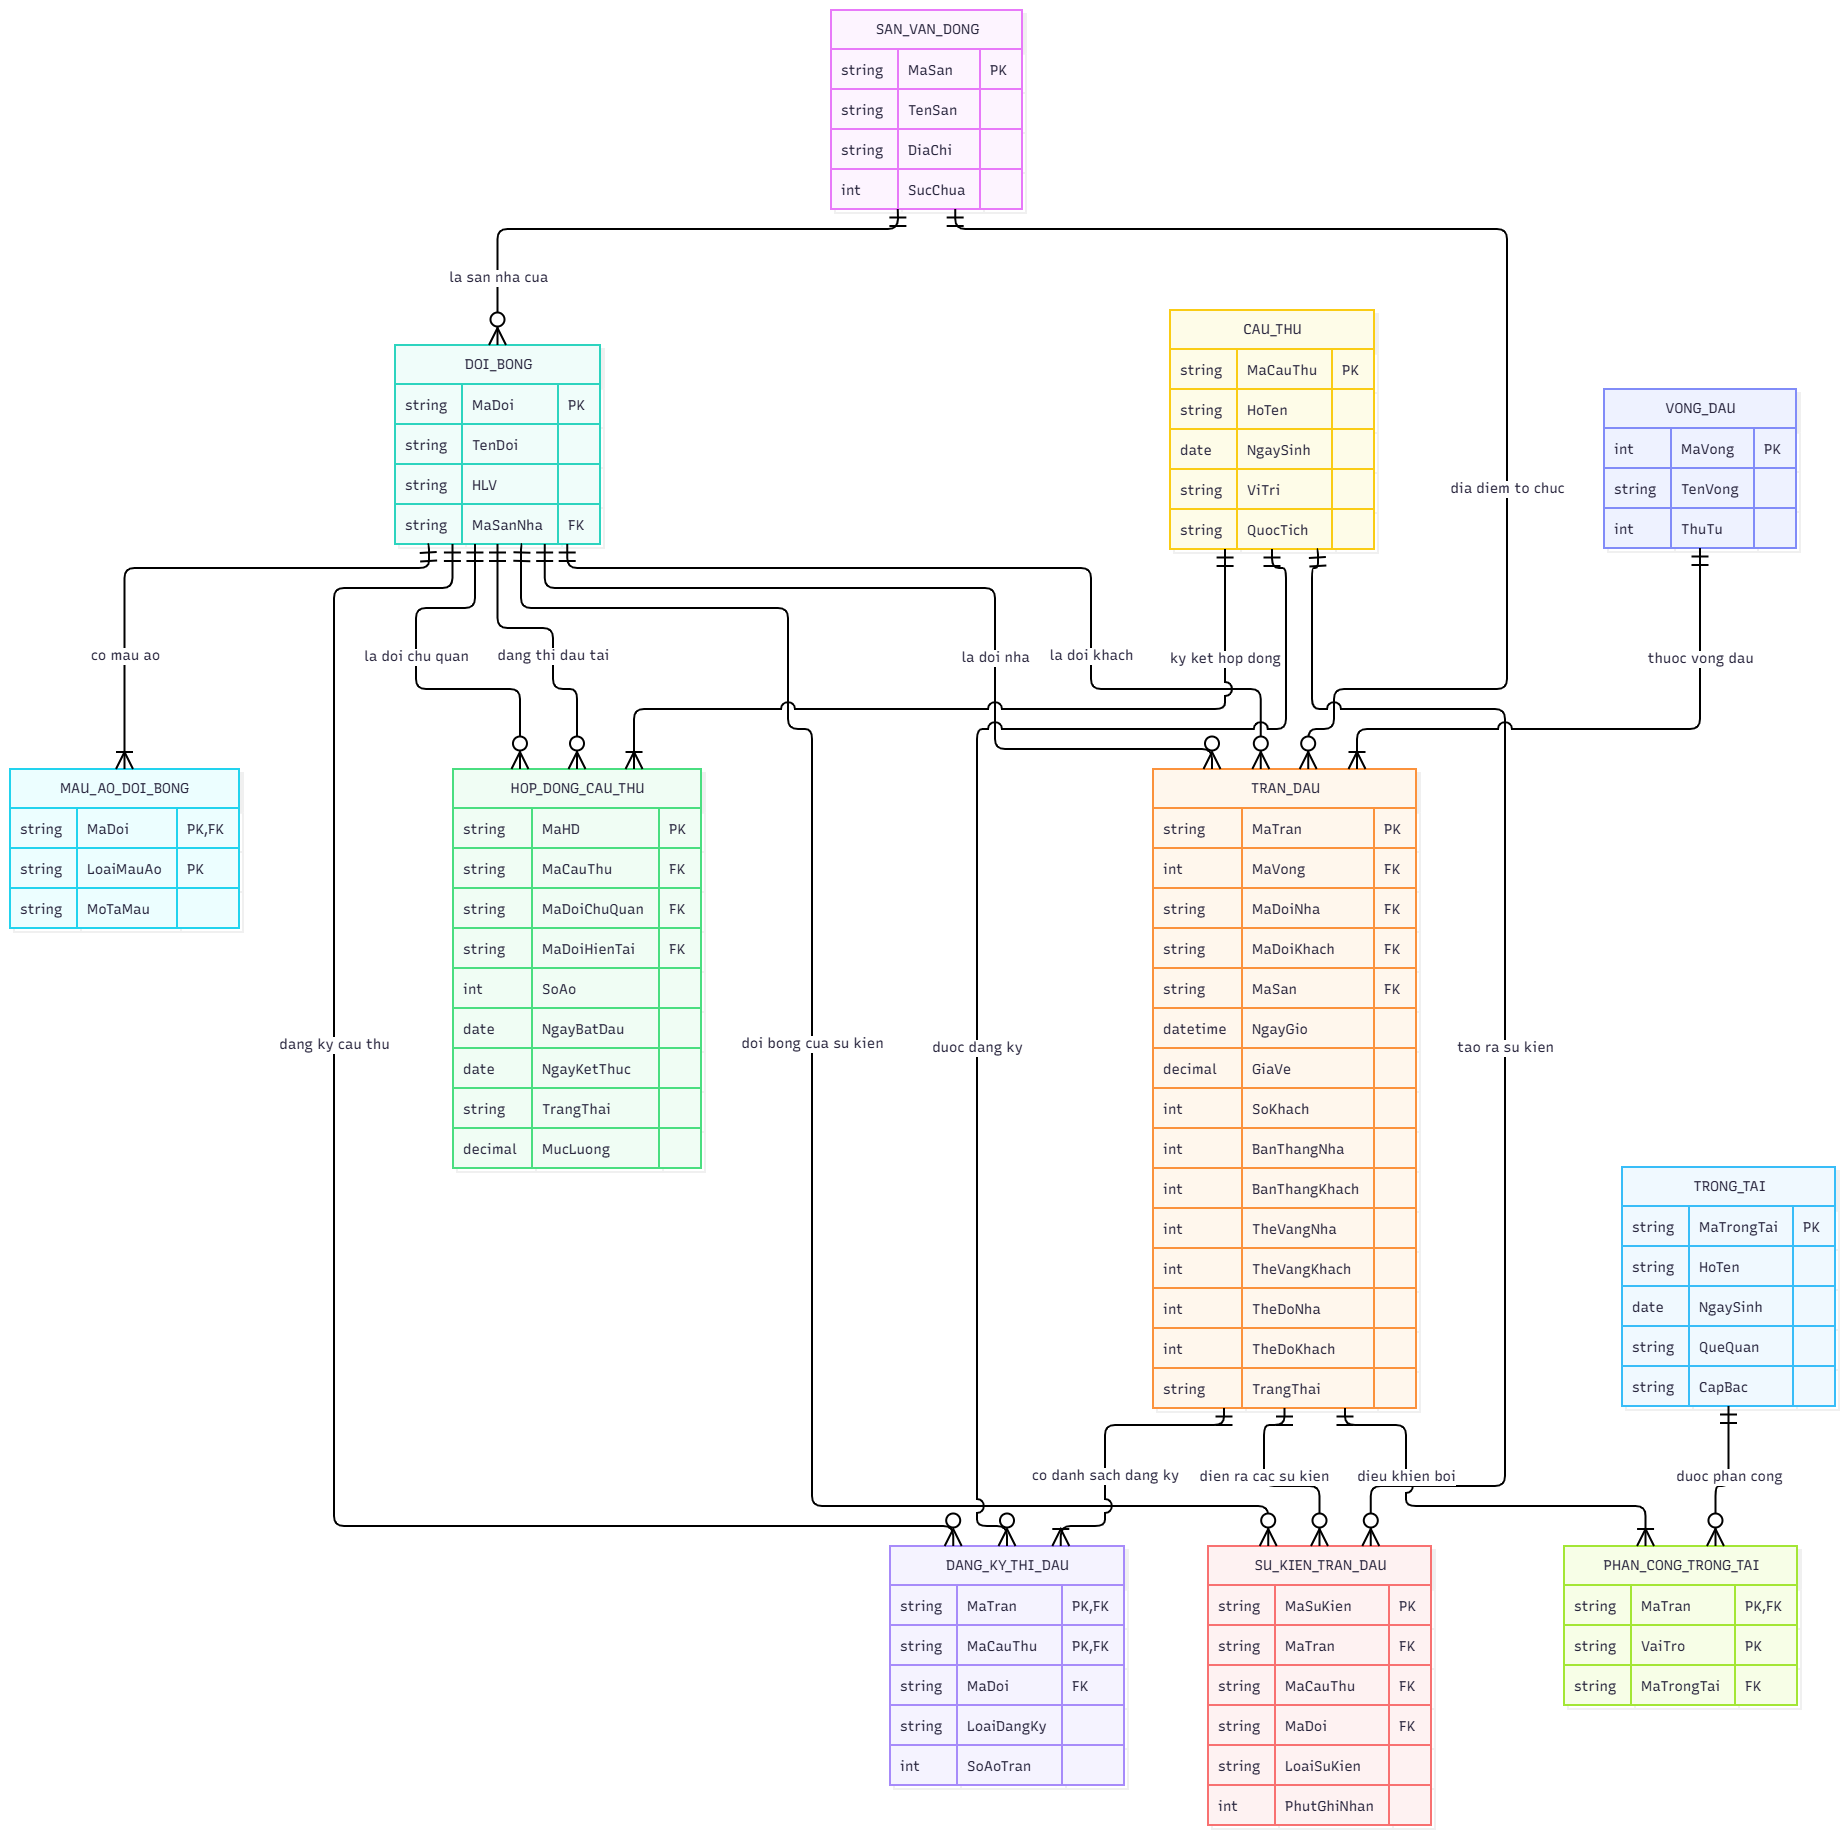
\includegraphics[angle=90, width=0.7\textheight, keepaspectratio]{Figures/RSD.png}
    \caption{Sơ đồ cấu trúc lược đồ quan hệ và mối liên kết khóa}
    \label{fig:relational_diagram}
\end{figure}

\section{Xác định phụ thuộc hàm và chứng minh chuẩn BCNF cho từng lược đồ}

\subsection{Quan hệ SAN\_VAN\_DONG}
\begin{itemize}
    \item Tập thuộc tính: $U = \{\text{MaSan}, \text{TenSan}, \text{DiaChi}, \text{SucChua}\}$.
    \item Tập phụ thuộc hàm tối thiểu $F_1$:
    \begin{align*}
        f_{1.1}: & \quad \text{MaSan} \rightarrow \{\text{TenSan}, \text{DiaChi}, \text{SucChua}\} \\
        f_{1.2}: & \quad \text{TenSan} \rightarrow \{\text{MaSan}, \text{DiaChi}, \text{SucChua}\}
    \end{align*}
    \item Xác định khóa ứng viên:
    $$\text{MaSan}^+ = U \implies \text{MaSan} \text{ là khóa ứng viên.}$$
    $$\text{TenSan}^+ = U \implies \text{TenSan} \text{ là khóa ứng viên.}$$
    \item Kiểm tra điều kiện BCNF:
    \begin{itemize}
        \item Xét $f_{1.1}$: Vế trái $\text{MaSan}$ là siêu khóa.
        \item Xét $f_{1.2}$: Vế trái $\text{TenSan}$ là siêu khóa.
    \end{itemize}
    \item \textbf{Kết luận}: Quan hệ \texttt{SAN\_VAN\_DONG} đạt dạng chuẩn \textbf{BCNF}.
\end{itemize}

\subsection{Quan hệ DOI\_BONG}
\begin{itemize}
    \item Tập thuộc tính: $U = \{\text{MaDoi}, \text{TenDoi}, \text{HLV}, \text{MaSanNha}\}$.
    \item Tập phụ thuộc hàm $F_2$:
    \begin{align*}
        f_{2.1}: & \quad \text{MaDoi} \rightarrow \{\text{TenDoi}, \text{HLV}, \text{MaSanNha}\} \\
        f_{2.2}: & \quad \text{TenDoi} \rightarrow \{\text{MaDoi}, \text{HLV}, \text{MaSanNha}\}
    \end{align*}
    \item Xác định khóa: Khóa ứng viên gồm $\{\text{MaDoi}\}$ và $\{\text{TenDoi}\}$.
    \item Kiểm tra điều kiện BCNF: Cả hai vế trái $\text{MaDoi}$ và $\text{TenDoi}$ đều là siêu khóa của quan hệ.
    \item \textbf{Kết luận}: Quan hệ \texttt{DOI\_BONG} đạt dạng chuẩn \textbf{BCNF}.
\end{itemize}

\subsection{Quan hệ MAU\_AO\_DOI\_BONG}
\begin{itemize}
    \item Tập thuộc tính: $U = \{\text{MaDoi}, \text{LoaiMauAo}, \text{MoTaMau}\}$.
    \item Tập phụ thuộc hàm $F_3$:
    $$f_{3.1}: \quad \{\text{MaDoi}, \text{LoaiMauAo}\} \rightarrow \text{MoTaMau}$$
    \item Khóa ứng viên: $K = \{\text{MaDoi}, \text{LoaiMauAo}\}$ do $\{\text{MaDoi}, \text{LoaiMauAo}\}^+ = U$.
    \item Kiểm tra điều kiện BCNF: Vế trái của phụ thuộc hàm $f_{3.1}$ là khóa chính của quan hệ.
    \item \textbf{Kết luận}: Quan hệ \texttt{MAU\_AO\_DOI\_BONG} đạt dạng chuẩn \textbf{BCNF}.
\end{itemize}

\subsection{Quan hệ CAU\_THU}
\begin{itemize}
    \item Tập thuộc tính: $U = \{\text{MaCauThu}, \text{HoTen}, \text{NgaySinh}, \text{ViTri}, \text{QuocTich}\}$.
    \item Tập phụ thuộc hàm $F_4$:
    $$f_{4.1}: \quad \text{MaCauThu} \rightarrow \{\text{HoTen}, \text{NgaySinh}, \text{ViTri}, \text{QuocTich}\}$$
    \item Khóa ứng viên: $K = \{\text{MaCauThu}\}$.
    \item Kiểm tra điều kiện BCNF: Vế trái $\text{MaCauThu}$ là siêu khóa.
    \item \textbf{Kết luận}: Quan hệ \texttt{CAU\_THU} đạt dạng chuẩn \textbf{BCNF}.
\end{itemize}

\subsection{Quan hệ HOP\_DONG\_CAU\_THU}
\begin{itemize}
    \item Tập thuộc tính: $U = \{\text{MaHD}, \text{MaCauThu}, \text{MaDoiChuQuan}, \text{MaDoiHienTai}, \text{SoAo}, \text{NgayBatDau}, \text{NgayKetThuc}, \text{TrangThai}, \text{MucLuong}\}$.
    \item Tập phụ thuộc hàm $F_5$:
    $$f_{5.1}: \quad \text{MaHD} \rightarrow \{\text{MaCauThu}, \text{MaDoiChuQuan}, \text{MaDoiHienTai}, \text{SoAo}, \text{NgayBatDau}, \text{NgayKetThuc}, \text{TrangThai}, \text{MucLuong}\}$$
    \item Khóa ứng viên: $K = \{\text{MaHD}\}$.
    \item Kiểm tra điều kiện BCNF: Vế trái $\text{MaHD}$ là siêu khóa duy nhất.
    \item \textbf{Kết luận}: Quan hệ \texttt{HOP\_DONG\_CAU\_THU} đạt dạng chuẩn \textbf{BCNF}.
\end{itemize}

\subsection{Quan hệ TRONG\_TAI}
\begin{itemize}
    \item Tập thuộc tính: $U = \{\text{MaTrongTai}, \text{HoTen}, \text{NgaySinh}, \text{QueQuan}, \text{CapBac}\}$.
    \item Tập phụ thuộc hàm $F_6$:
    $$f_{6.1}: \quad \text{MaTrongTai} \rightarrow \{\text{HoTen}, \text{NgaySinh}, \text{QueQuan}, \text{CapBac}\}$$
    \item Khóa ứng viên: $K = \{\text{MaTrongTai}\}$.
    \item Kiểm tra điều kiện BCNF: Vế trái $\text{MaTrongTai}$ là siêu khóa.
    \item \textbf{Kết luận}: Quan hệ \texttt{TRONG\_TAI} đạt dạng chuẩn \textbf{BCNF}.
\end{itemize}

\subsection{Quan hệ VONG\_DAU}
\begin{itemize}
    \item Tập thuộc tính: $U = \{\text{MaVong}, \text{TenVong}, \text{ThuTu}\}$.
    \item Tập phụ thuộc hàm $F_7$:
    \begin{align*}
        f_{7.1}: & \quad \text{MaVong} \rightarrow \{\text{TenVong}, \text{ThuTu}\} \\
        f_{7.2}: & \quad \text{ThuTu} \rightarrow \{\text{MaVong}, \text{TenVong}\}
    \end{align*}
    \item Khóa ứng viên: $K_1 = \{\text{MaVong}\}$, $K_2 = \{\text{ThuTu}\}$.
    \item Kiểm tra điều kiện BCNF: Vế trái của cả hai phụ thuộc hàm đều là siêu khóa.
    \item \textbf{Kết luận}: Quan hệ \texttt{VONG\_DAU} đạt dạng chuẩn \textbf{BCNF}.
\end{itemize}

\subsection{Quan hệ TRAN\_DAU}
\begin{itemize}
    \item Tập thuộc tính:
    $$U = \{\text{MaTran}, \text{MaVong}, \text{MaDoiNha}, \text{MaDoiKhach}, \text{MaSan}, \text{NgayGio}, \text{GiaVe}, \text{SoKhach}, \text{BanThangNha}, \text{BanThangKhach}, \dots\}$$
    \item Tập phụ thuộc hàm $F_8$:
    \begin{align*}
        f_{8.1}: & \quad \text{MaTran} \rightarrow U \setminus \{\text{MaTran}\} \\
        f_{8.2}: & \quad \{\text{MaDoiNha}, \text{MaDoiKhach}\} \rightarrow U \setminus \{\text{MaDoiNha}, \text{MaDoiKhach}\}
    \end{align*}
    (Do mỗi cặp đối đầu sân nhà -- sân khách chỉ diễn ra duy nhất một trận trong cả mùa giải).
    \item Khóa ứng viên: $K_1 = \{\text{MaTran}\}$, $K_2 = \{\text{MaDoiNha}, \text{MaDoiKhach}\}$.
    \item Kiểm tra điều kiện BCNF: Cả hai vế trái $\text{MaTran}$ và $\{\text{MaDoiNha}, \text{MaDoiKhach}\}$ đều là siêu khóa.
    \item \textbf{Kết luận}: Quan hệ \texttt{TRAN\_DAU} đạt dạng chuẩn \textbf{BCNF}.
\end{itemize}

\subsection{Quan hệ PHAN\_CONG\_TRONG\_TAI}
\begin{itemize}
    \item Tập thuộc tính: $U = \{\text{MaTran}, \text{VaiTro}, \text{MaTrongTai}\}$.
    \item Tập phụ thuộc hàm $F_9$:
    \begin{align*}
        f_{9.1}: & \quad \{\text{MaTran}, \text{VaiTro}\} \rightarrow \text{MaTrongTai} \\
        f_{9.2}: & \quad \{\text{MaTran}, \text{MaTrongTai}\} \rightarrow \text{VaiTro}
    \end{align*}
    (Trong một trận đấu, mỗi vai trò chỉ có đúng một trọng tài; và mỗi trọng tài chỉ đảm nhiệm tối đa một vai trò).
    \item Khóa ứng viên: $K_1 = \{\text{MaTran}, \text{VaiTro}\}$, $K_2 = \{\text{MaTran}, \text{MaTrongTai}\}$.
    \item Kiểm tra điều kiện BCNF: Vế trái của $f_{9.1}$ và $f_{9.2}$ đều là siêu khóa của quan hệ.
    \item \textbf{Kết luận}: Quan hệ \texttt{PHAN\_CONG\_TRONG\_TAI} đạt dạng chuẩn \textbf{BCNF}.
\end{itemize}

\subsection{Quan hệ DANG\_KY\_THI\_DAU}
\begin{itemize}
    \item Tập thuộc tính: $U = \{\text{MaTran}, \text{MaCauThu}, \text{MaDoi}, \text{LoaiDangKy}, \text{SoAoTran}\}$.
    \item Tập phụ thuộc hàm $F_{10}$:
    $$f_{10.1}: \quad \{\text{MaTran}, \text{MaCauThu}\} \rightarrow \{\text{MaDoi}, \text{LoaiDangKy}, \text{SoAoTran}\}$$
    \item Khóa ứng viên: $K = \{\text{MaTran}, \text{MaCauThu}\}$.
    \item Kiểm tra điều kiện BCNF: Vế trái $\{\text{MaTran}, \text{MaCauThu}\}$ là siêu khóa duy nhất.
    \item \textbf{Kết luận}: Quan hệ \texttt{DANG\_KY\_THI\_DAU} đạt dạng chuẩn \textbf{BCNF}.
\end{itemize}

\subsection{Quan hệ SU\_KIEN\_TRAN\_DAU}
\begin{itemize}
    \item Tập thuộc tính: $U = \{\text{MaSuKien}, \text{MaTran}, \text{MaCauThu}, \text{MaDoi}, \text{LoaiSuKien}, \text{PhutGhiNhan}\}$.
    \item Tập phụ thuộc hàm $F_{11}$:
    $$f_{11.1}: \quad \text{MaSuKien} \rightarrow \{\text{MaTran}, \text{MaCauThu}, \text{MaDoi}, \text{LoaiSuKien}, \text{PhutGhiNhan}\}$$
    \item Khóa ứng viên: $K = \{\text{MaSuKien}\}$.
    \item Kiểm tra điều kiện BCNF: Vế trái $\text{MaSuKien}$ là siêu khóa.
    \item \textbf{Kết luận}: Quan hệ \texttt{SU\_KIEN\_TRAN\_DAU} đạt dạng chuẩn \textbf{BCNF}.
\end{itemize}

% \section{Phân tích thuật toán tách chuẩn BCNF}

% Mục này trình bày một ví dụ thiết kế chưa chuẩn hóa và các bước áp dụng thuật toán tách để đưa quan hệ về dạng chuẩn BCNF.

% \subsection{Tình huống thiết kế vi phạm chuẩn hóa}
% Giả sử người thiết kế gộp chung thông tin của Trận đấu và Sân vận động vào trong một bảng duy nhất:
% $$R_{\text{Gop}}(\underline{\text{MaTran}}, \text{NgayGio}, \text{MaSan}, \text{TenSan}, \text{DiaChi}, \text{SucChua})$$

% Tập phụ thuộc hàm trên $R_{\text{Gop}}$ gồm:
% \begin{align*}
%     f_1: & \quad \text{MaTran} \rightarrow \{\text{NgayGio}, \text{MaSan}, \text{TenSan}, \text{DiaChi}, \text{SucChua}\} \\
%     f_2: & \quad \text{MaSan} \rightarrow \{\text{TenSan}, \text{DiaChi}, \text{SucChua}\}
% \end{align*}

% \paragraph{Phân tích vi phạm BCNF:}
% \begin{itemize}
%     \item Khóa chính duy nhất của $R_{\text{Gop}}$ là $\{\text{MaTran}\}$.
%     \item Xét phụ thuộc hàm $f_2: \text{MaSan} \rightarrow \{\text{TenSan}, \text{DiaChi}, \text{SucChua}\}$. Vế trái $\text{MaSan}$ không phải là siêu khóa của $R_{\text{Gop}}$ (vì bao đóng của $\text{MaSan}$ không chứa thuộc tính $\text{MaTran}$ và $\text{NgayGio}$).
%     \item Do đó, quan hệ $R_{\text{Gop}}$ vi phạm định nghĩa dạng chuẩn BCNF và vi phạm dạng chuẩn 3 do tồn tại phụ thuộc bắc cầu.
%     \item Hậu quả là thông tin tên sân, địa chỉ, sức chứa bị lặp lại ở mọi trận đấu diễn ra trên sân đó, dẫn đến các dị thường khi thêm, sửa hoặc xóa dữ liệu.
% \end{itemize}

% \subsection{Các bước thực hiện thuật toán tách BCNF}
% Thuật toán tách được thực hiện như sau:
% \begin{itemize}
%     \item \textbf{Bước 1}: Chọn phụ thuộc hàm vi phạm điều kiện BCNF là $f_2: \text{MaSan} \rightarrow \{\text{TenSan}, \text{DiaChi}, \text{SucChua}\}$.
%     \item \textbf{Bước 2}: Tách $R_{\text{Gop}}$ thành hai lược đồ quan hệ con $R_1$ và $R_2$:
%     $$R_1 = \{\underline{\mathbf{MaSan}}, \text{TenSan}, \text{DiaChi}, \text{SucChua}\} \equiv \text{SAN\_VAN\_DONG}$$
%     $$R_2 = \{\underline{\mathbf{MaTran}}, \text{NgayGio}, \textit{MaSan}\} \equiv \text{TRAN\_DAU\_RUT\_GON}$$
%     \item \textbf{Bước 3}: Kiểm tra các tính chất của phép tách:
%     \begin{enumerate}
%         \item \textit{Tính kết nối không mất mát thông tin}:
%         Giao của hai quan hệ là $R_1 \cap R_2 = \{\text{MaSan}\}$. Vì $\text{MaSan}$ là khóa chính của $R_1$ nên phép tách bảo toàn toàn bộ dữ liệu ban đầu:
%         $$R_{\text{Gop}} = R_1 \bowtie R_2.$$
%         \item \textit{Tính bảo toàn phụ thuộc hàm}: Các phụ thuộc hàm trong tập ban đầu đều được duy trì trong các bảng con.
%         \item \textit{Kiểm tra lại điều kiện BCNF}: Cả hai quan hệ $R_1$ và $R_2$ đều thỏa mãn dạng chuẩn BCNF.
%     \end{enumerate}
% \end{itemize}

% Kết quả này cho thấy việc tách các thực thể theo mô hình thiết kế đã loại bỏ hoàn toàn dư thừa dữ liệu.
